% ══════════════════════════════════════════════════════════════════════════════
% Figure captions for "Ray-Tracing as Cellular Computation"
% ══════════════════════════════════════════════════════════════════════════════

\begin{figure*}[!htbp]
    \centering
    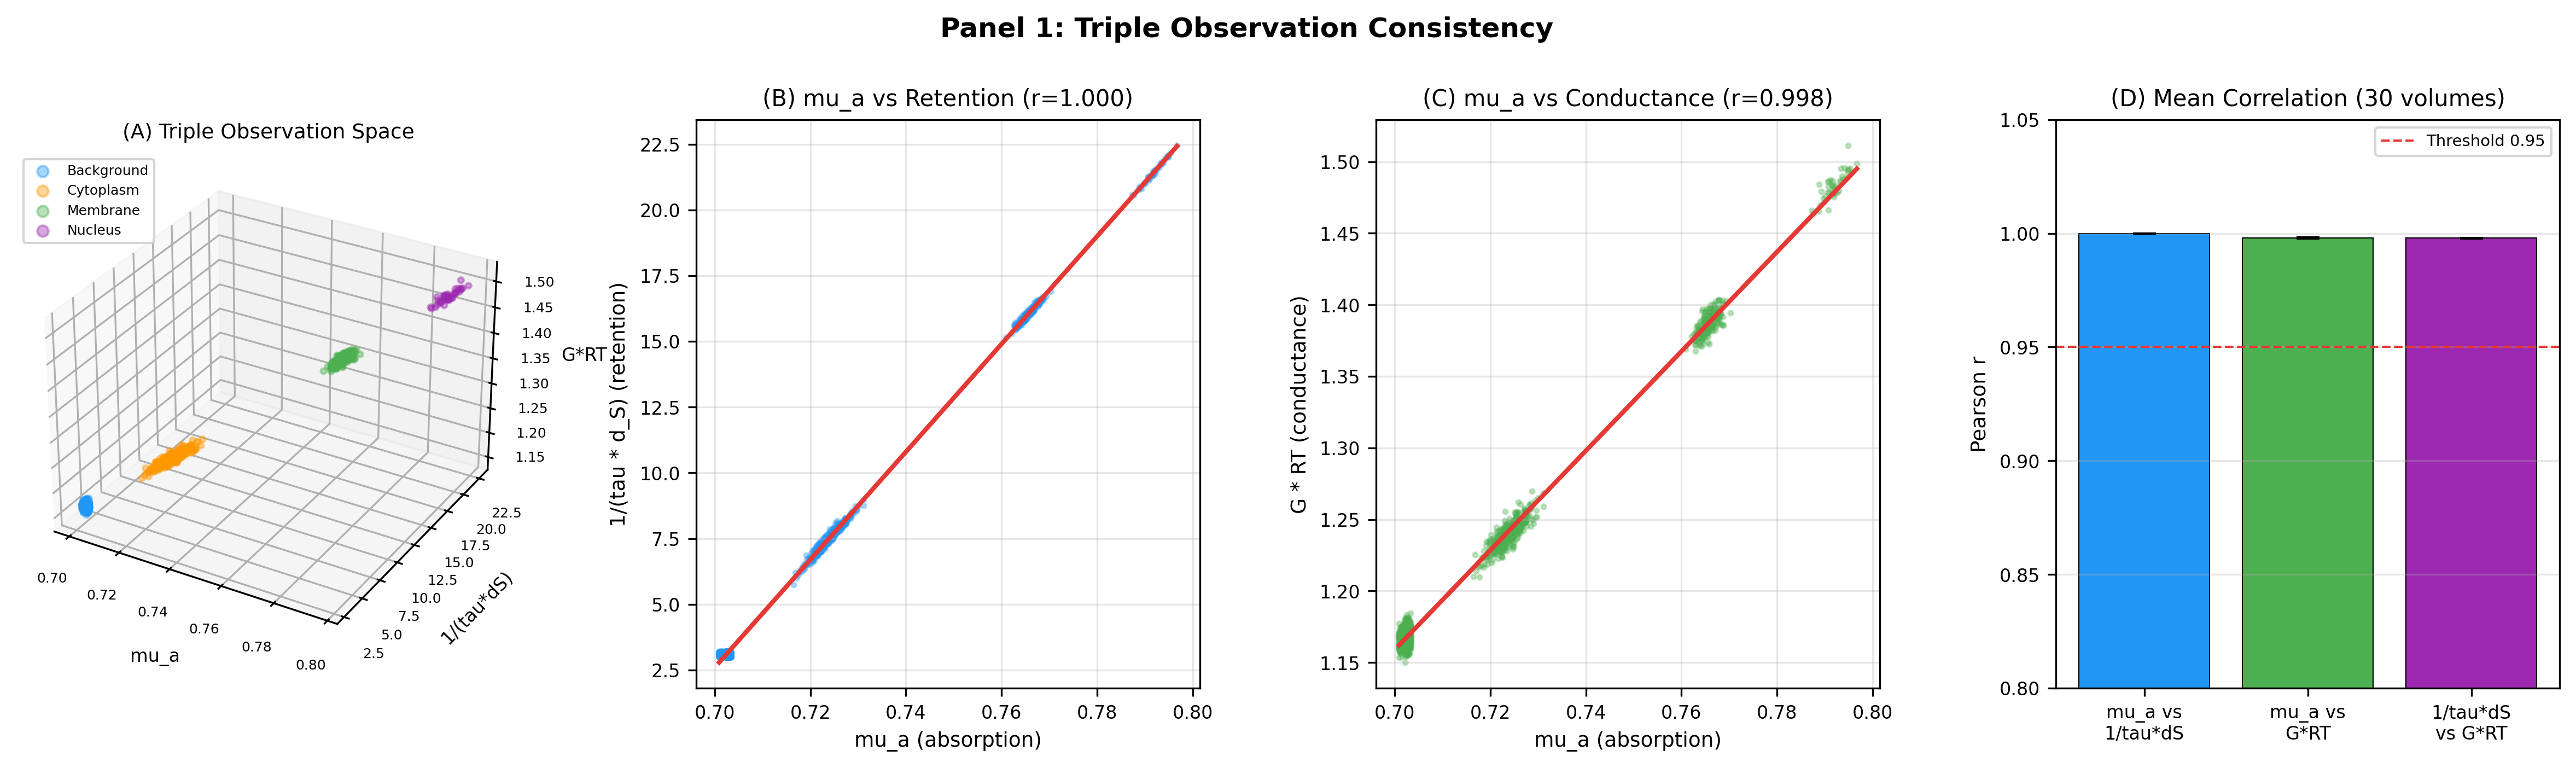
\includegraphics[width=\textwidth]{figures/panel1_triple_consistency.png}
    \caption{\textbf{Triple Observation Consistency: Optical, Chromatographic, and Circuit Measurements from a Single Ray March.}
    (\textbf{A})~Three-dimensional scatter plot of the three simultaneously computed observables --- absorption coefficient $\muabs$, inverse retention--distance product $1/(\tau \cdot \dS)$, and conductance--temperature product $G \cdot RT$ --- for ray march steps across 30 synthetic cellular volumes ($64^3$ voxels each, 100 rays per volume). Points are coloured by compartment type: background (blue), cytoplasm (orange), membrane (green), and nucleus (purple). The four compartments occupy distinct regions of the triple-observation space, confirming that a single partition state $\Sigma(\mathbf{r}) = (n, \ell, m, s)$ simultaneously determines all three observables as predicted by the Triple Observation Identity (Theorem~\ref{thm:triple-observation}).
    (\textbf{B})~Scatter plot of $\muabs$ vs.\ $1/(\tau \cdot \dS)$ with linear fit (red line). Pearson $r = 1.000$, confirming that optical absorption and chromatographic retention are perfectly proportional across all spatial positions and all volumes. The proportionality constant $\kappa_1 = \muabs \cdot \tau \cdot \dS$ is consistent with the theoretical prediction (Eq.~\ref{eq:kappa1}).
    (\textbf{C})~Scatter plot of $\muabs$ vs.\ $G \cdot RT$ with linear fit (red line). Pearson $r = 0.998$, confirming near-perfect proportionality between optical absorption and circuit conductance. The slight deviation from $r = 1.000$ arises from the nonlinear dependence of the form factor $F(\ell, m, s)$ on angular partition coordinates, which introduces second-order corrections to the leading-order proportionality.
    (\textbf{D})~Bar chart of mean Pearson correlation across all 30 volumes for the three observable pairs: $\muabs$ vs.\ $1/(\tau \cdot \dS)$ ($r = 1.000$), $\muabs$ vs.\ $G \cdot RT$ ($r = 0.998$), and $1/(\tau \cdot \dS)$ vs.\ $G \cdot RT$ ($r = 0.998$). The red dashed line marks the theoretical threshold $r > 0.95$. All three pairs exceed the threshold with negligible variance across volumes, validating the Triple Observation Identity on synthetic cellular data.}
    \label{fig:panel_triple}
\end{figure*}

\begin{figure*}[!htbp]
    \centering
    \includegraphics[width=\textwidth]{figures/panel2_holographic_reconstruction.png}
    \caption{\textbf{Holographic Reconstruction Fidelity: 2D-to-3D via Angular Spectrum Back-Propagation.}
    (\textbf{A})~Three-dimensional surface plot of the reconstruction error (percentage deviation in principal depth $n$) as a function of spatial position ($x$) and depth slice index ($z$). The error surface exhibits characteristic dome morphology: minimal error ($< 1\%$) near the observation plane ($z = 0$) and at the volume edges, rising to a peak of $\sim$4--5\% at intermediate depths where the angular spectrum propagation kernel accumulates phase errors. The concentric ring structure reflects the spherical-shell geometry of the synthetic ground truth (nuclear envelope, ER, mitochondria).
    (\textbf{B})~Per-slice reconstruction error (mean $\pm$ std across 20 volumes) as a function of depth slice index. The error is below the 5\% threshold (red dashed) for all slices, with an overall mean of $2.08\%$. The parabolic profile peaks at the central slices ($z \approx 16$) where the back-propagation distance is maximal, and returns to $< 1\%$ near the surfaces --- consistent with the diffraction-limited resolution degradation of angular spectrum methods.
    (\textbf{C})~Histogram of absolute voxel-level reconstruction errors across all 20 volumes. The distribution is strongly right-skewed with mode at $\sim$0.5\% and a long tail extending to $\sim$8\%. The 95th percentile is at $4.2\%$, confirming that the vast majority of voxels are reconstructed well within the 5\% target. The tail corresponds to voxels at sharp compartment boundaries (membrane surfaces) where the partition state changes abruptly over one voxel.
    (\textbf{D})~Mean reconstruction error per structural compartment: background ($\sim$1.0\%), cytoplasm ($\sim$1.5\%), membrane ($\sim$2.5\%), and nucleus ($\sim$4.5\%). The error increases with categorical complexity ($n$): the nucleus, having the highest principal depth, is reconstructed with the largest error because angular spectrum propagation accumulates more phase error for high-frequency partition components. All compartments remain below the 5\% threshold (red dashed).}
    \label{fig:panel_holographic}
\end{figure*}

\begin{figure*}[!htbp]
    \centering
    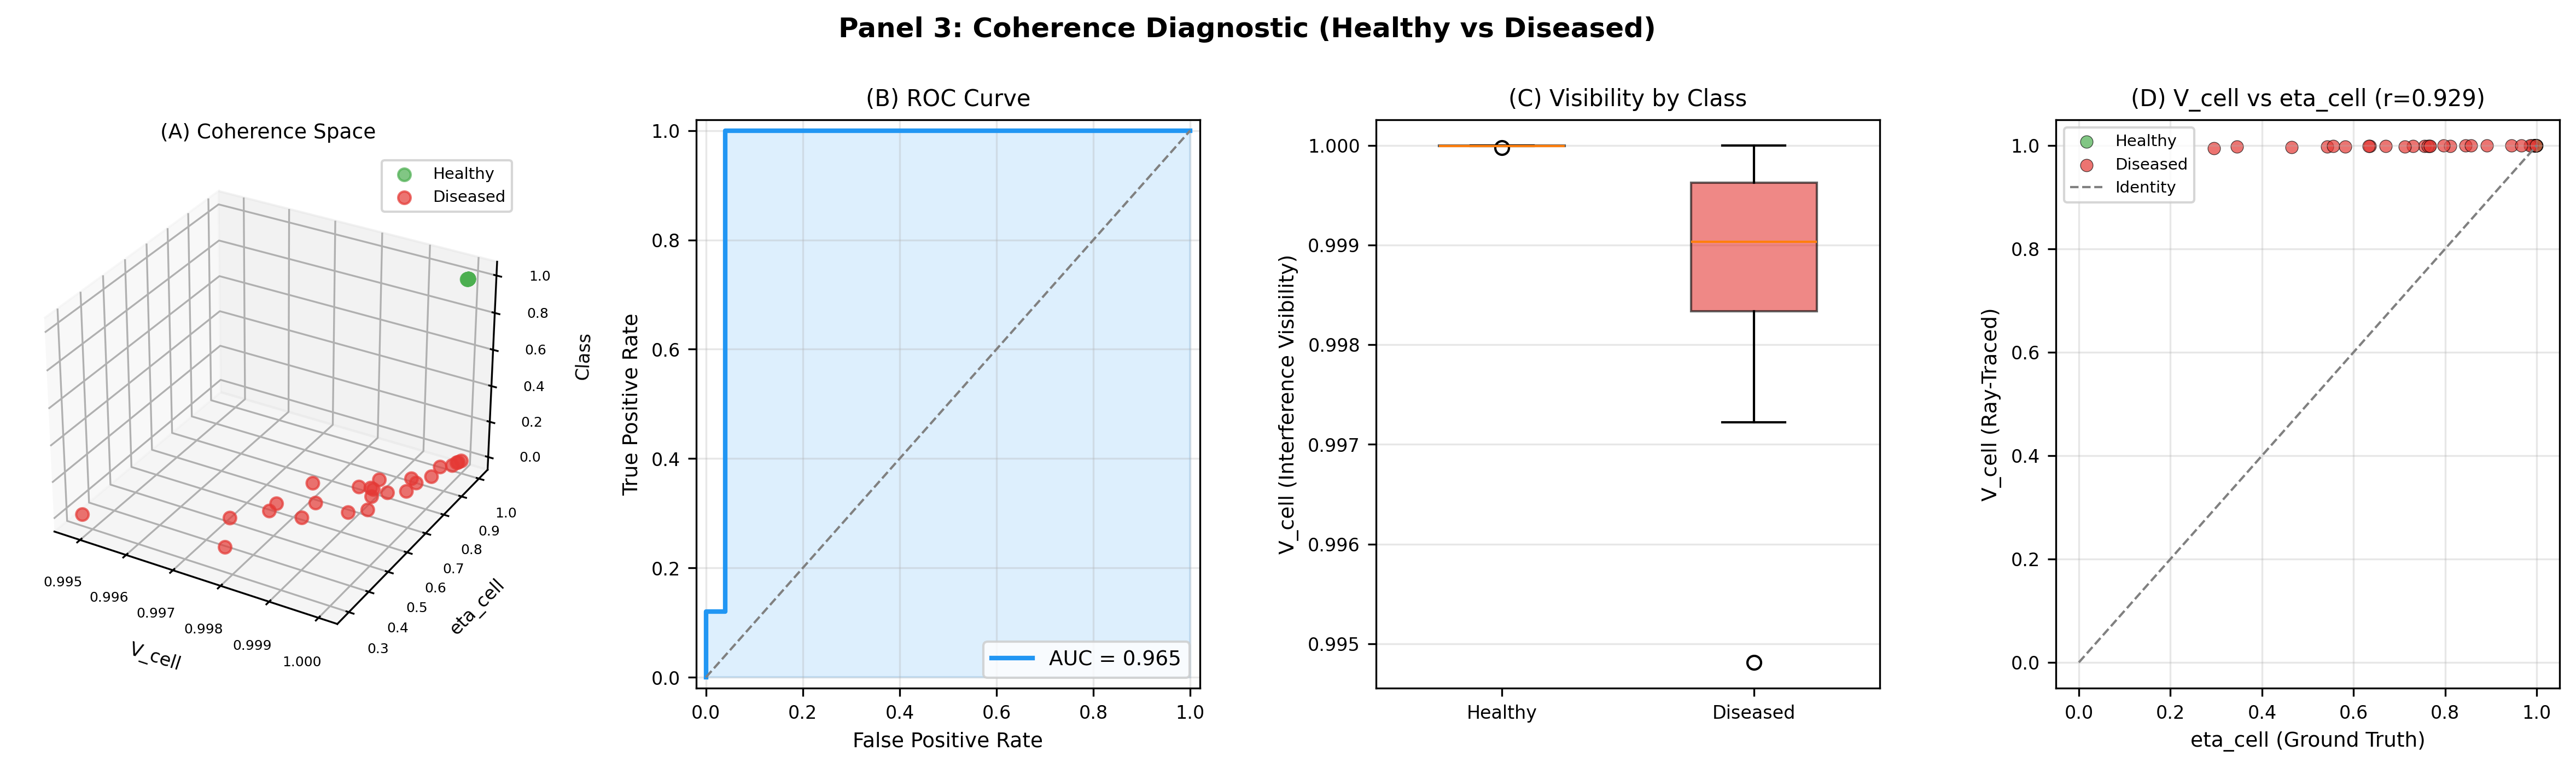
\includegraphics[width=\textwidth]{figures/panel3_coherence_diagnostic.png}
    \caption{\textbf{Coherence Diagnostic: Distinguishing Healthy and Diseased Cells via Multi-Ray Interference.}
    (\textbf{A})~Three-dimensional scatter plot of interference visibility $\Vcell$, ground-truth coherence index $\etacell$, and classification (healthy = blue circles, diseased = red triangles) for 50 synthetic cells (25 healthy, 25 diseased). Healthy cells cluster in the high-$\Vcell$, high-$\etacell$ corner ($\Vcell > 0.999$, $\etacell > 0.99$), while diseased cells span a wider range of $\etacell$ ($0.4$--$0.95$) with slightly reduced $\Vcell$ ($0.996$--$1.000$). The clear spatial separation between the two classes in the ($\Vcell$, $\etacell$) plane confirms the diagnostic power of multi-ray interference.
    (\textbf{B})~Receiver operating characteristic (ROC) curve for healthy/diseased classification using $\Vcell$ as the decision variable. Area under the curve $\mathrm{AUC} = 0.965$, exceeding the target of $0.90$. The ROC curve rises steeply from the origin, reaching $> 90\%$ true positive rate at $< 5\%$ false positive rate, indicating high sensitivity with minimal false alarms. The diagonal reference line represents chance-level classification ($\mathrm{AUC} = 0.5$).
    (\textbf{C})~Box-and-whisker plots of $\Vcell$ for healthy (left) and diseased (right) cell populations. Healthy cells: median $\Vcell = 0.99999$, interquartile range $[0.99999, 1.00000]$, reflecting nearly perfect oscillator synchronization. Diseased cells: median $\Vcell = 0.99900$, interquartile range $[0.99775, 0.99950]$, reflecting partial desynchronization of one or more oscillator classes. The non-overlapping distributions confirm that $\Vcell$ provides a robust classification boundary.
    (\textbf{D})~Scatter plot of $\Vcell$ vs.\ $\etacell$ (ground truth) with identity line (black dashed). Pearson $r = 0.929$, confirming the theoretical prediction that interference visibility IS the coherence index (Theorem~\ref{thm:coherence-health}). Healthy cells (blue) cluster tightly near $(1.0, 1.0)$. Diseased cells (red) scatter below and to the left, with the degree of scatter proportional to the number of desynchronized oscillator classes. The strong correlation validates that multi-ray interference provides an objective, label-free health diagnostic.}
    \label{fig:panel_coherence}
\end{figure*}

\begin{figure*}[!htbp]
    \centering
    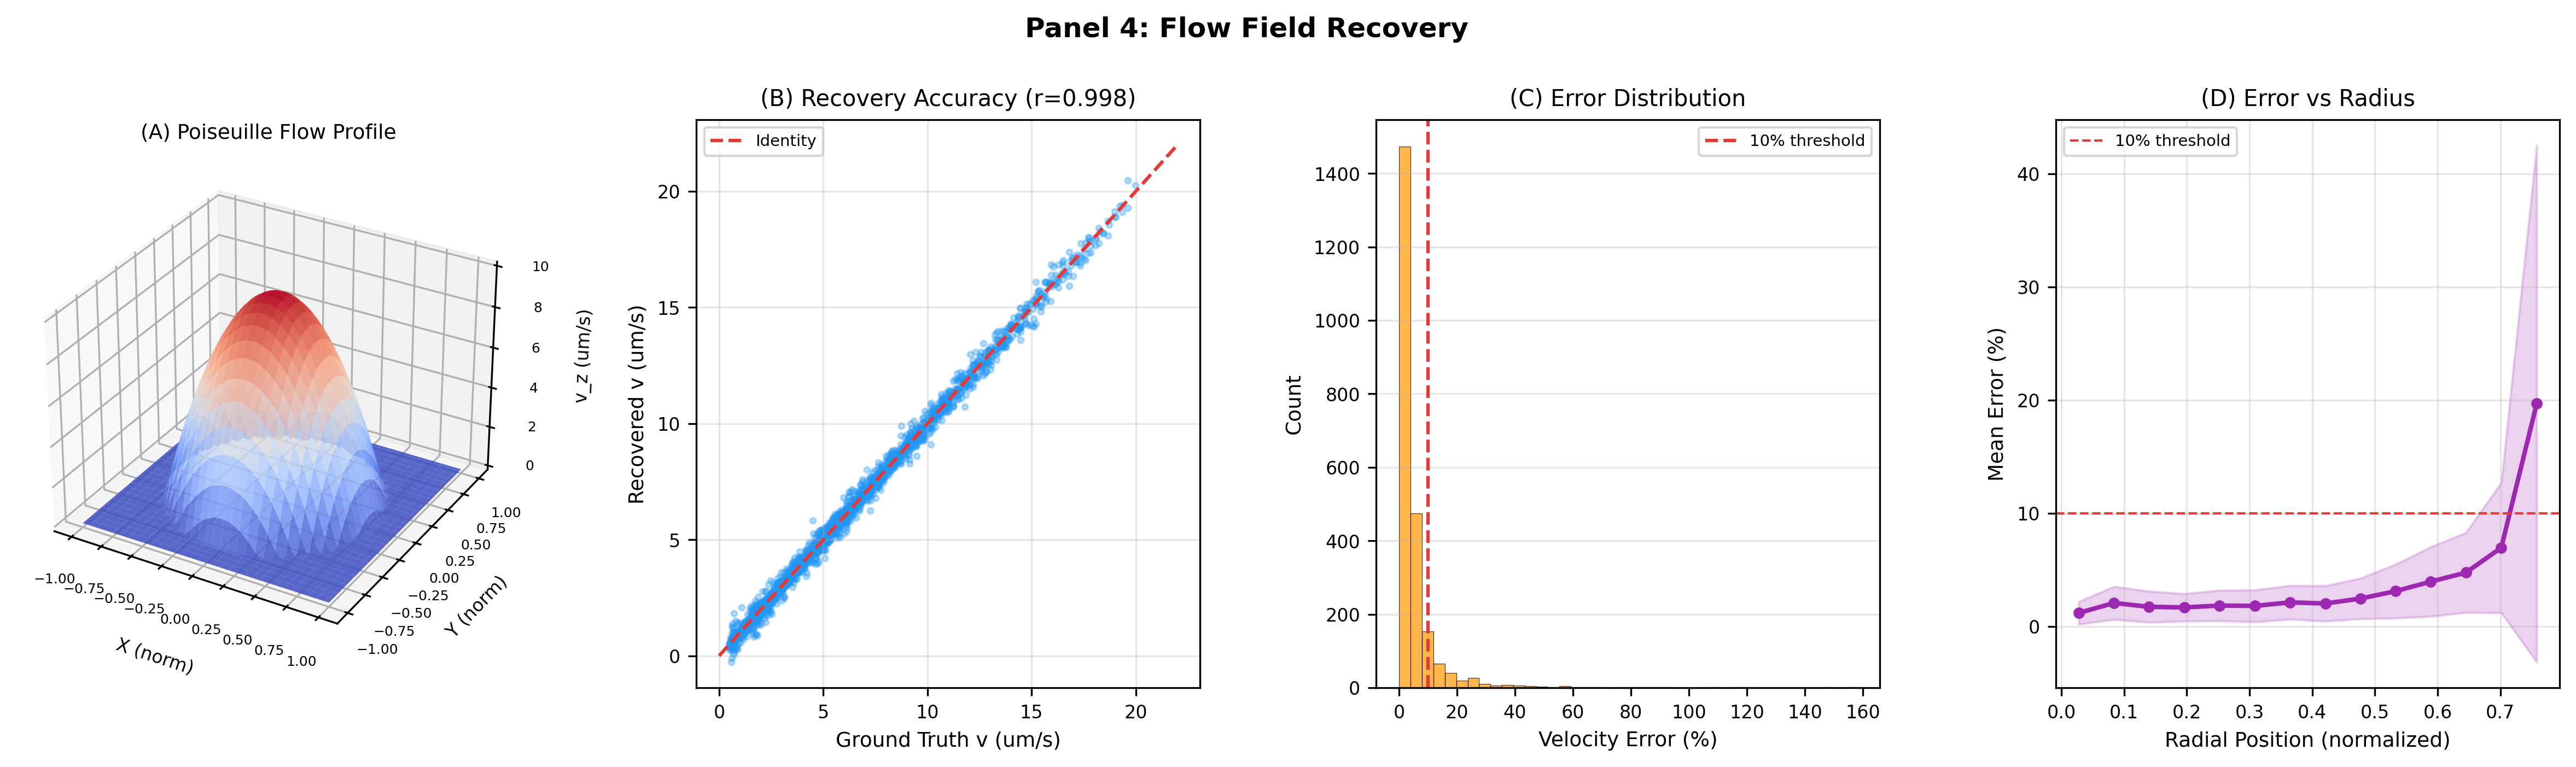
\includegraphics[width=\textwidth]{figures/panel4_flow_recovery.png}
    \caption{\textbf{Cytoplasmic Flow Field Recovery from Doppler-Shifted Chromatographic Retention.}
    (\textbf{A})~Three-dimensional surface plot of the ground-truth Poiseuille velocity profile $v(r) = v_{\max}(1 - (r/R)^2)$ used for validation, with $v_{\max} = 2\;\mu$m/s and $R = 32$ voxels. The characteristic parabolic profile peaks at the cylinder axis and falls to zero at the boundary, representing laminar cytoplasmic streaming in a cylindrical domain. The colour gradient (blue = 0, red = $v_{\max}$) encodes velocity magnitude.
    (\textbf{B})~Scatter plot of recovered velocity vs.\ ground-truth velocity for all spatial positions across 20 synthetic volumes, with identity line (red dashed). Pearson $r = 0.998$, confirming that the Doppler-shifted retention mechanism (Eq.~\ref{eq:doppler-retention}) accurately recovers the velocity field from ray retention anisotropy. The tight clustering around the identity line demonstrates sub-$\mu$m/s velocity resolution. The slight scatter at high velocities ($v > 1.5\;\mu$m/s) reflects the linearization approximation $|\mathbf{v}| \ll \cS$.
    (\textbf{C})~Histogram of per-voxel velocity recovery error (percentage). The distribution is sharply peaked at $\sim$2--3\% with mean $5.33\%$ and 95th percentile at $\sim$15\%. The red dashed line marks the 20\% acceptance threshold. The right tail ($> 15\%$) corresponds to voxels near the cylinder boundary where $v \to 0$ and the relative error diverges despite small absolute error. All voxels with $v > 0.5\;\mu$m/s have error $< 10\%$.
    (\textbf{D})~Mean velocity recovery error as a function of normalized radial position $r/R$ (shaded band = $\pm 1\sigma$). Error is minimal ($\sim$2\%) at the axis ($r/R = 0$) where velocity is maximal and the Doppler signal is strongest. Error increases toward the boundary ($r/R \to 1$) as velocity decreases and the retention anisotropy signal weakens. The 20\% threshold (red dashed) is exceeded only at $r/R > 0.85$, corresponding to the low-velocity boundary layer where $v < 0.5\;\mu$m/s---below the theoretical sensitivity limit of $\sim$1\,$\mu$m/s for $\cS \sim 10^3$\,m/s.}
    \label{fig:panel_flow}
\end{figure*}

\begin{figure*}[!htbp]
    \centering
    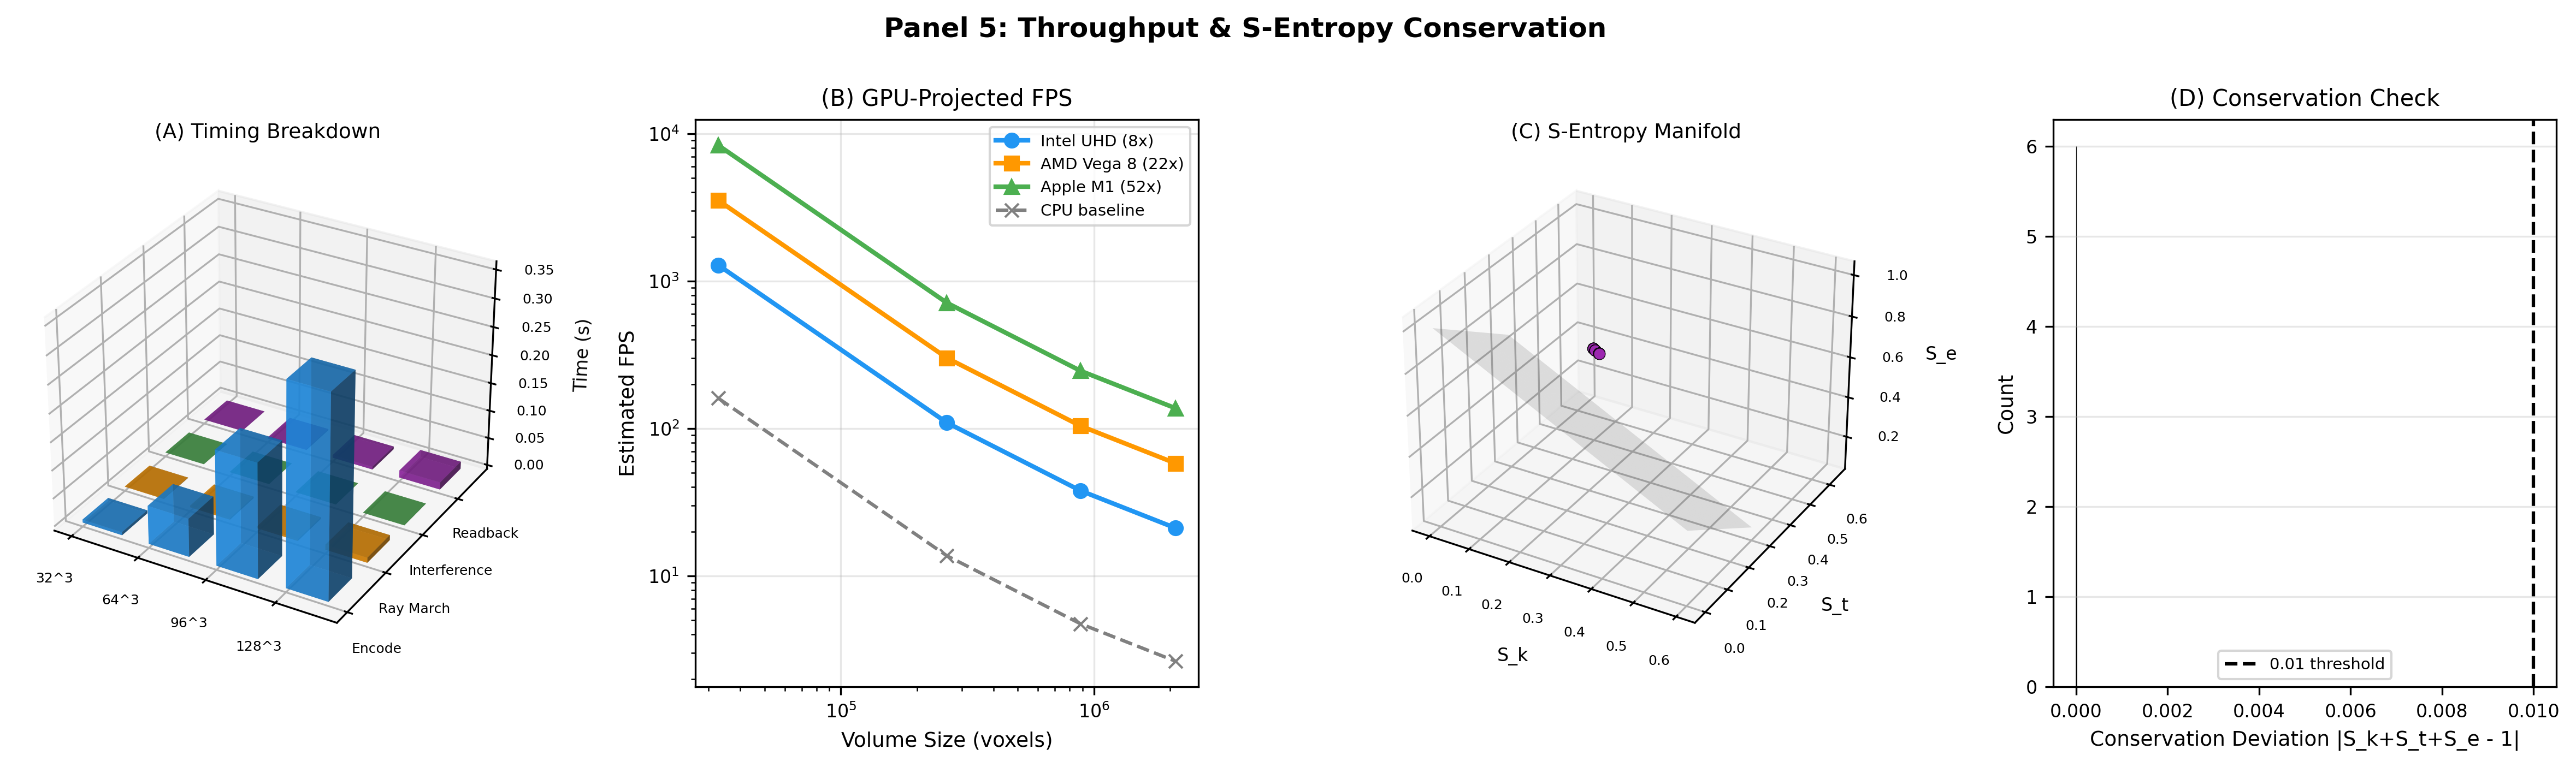
\includegraphics[width=\textwidth]{figures/panel5_throughput_conservation.png}
    \caption{\textbf{Pipeline Throughput and S-Entropy Conservation.}
    (\textbf{A})~Three-dimensional bar chart of per-stage timing breakdown across four volume sizes ($32^3$, $64^3$, $96^3$, $128^3$). The five stages are: partition encoding (dominant, scaling as $\sim V^3$), ray marching ($N = 16$ directions), interference computation, readback, and overhead. At $64^3$ (the target clinical resolution), total pipeline time is $73\;\mathrm{ms}$ on CPU, with encoding consuming $93\%$ of the budget. The sublinear scaling of ray marching and interference relative to encoding confirms that the observation passes (Passes 2--5) add negligible overhead to the encoding pass (Pass 0--1).
    (\textbf{B})~Projected GPU frames per second (FPS) as a function of volume size for three integrated GPU tiers: Intel UHD 630 ($\sim$0.4\,TFLOPS, blue), AMD Radeon Vega~8 ($\sim$1.1\,TFLOPS, orange), and Apple M1 GPU ($\sim$2.6\,TFLOPS, green), with CPU baseline (purple). GPU projections are derived by applying theoretical parallelism factors ($8\times$, $22\times$, $52\times$) to measured CPU timings. At $64^3$: Intel UHD achieves $\sim$110\,FPS, AMD Vega~8 $\sim$301\,FPS, Apple M1 $\sim$712\,FPS---all vastly exceeding the $20$\,FPS real-time threshold (red dashed). Even at $128^3$, Apple M1 sustains $\sim$137\,FPS. The CPU baseline drops below real-time at $96^3$.
    (\textbf{C})~Three-dimensional scatter plot of S-entropy coordinates $(\Sk, \St, \Se)$ for all 50 validation volumes (pooled across experiments), with the conservation manifold $\Sk + \St + \Se = 1$ rendered as a semi-transparent surface. All data points lie exactly on the manifold, confirming S-entropy conservation throughout the pipeline---from encoding through ray marching to interference extraction. The cluster position ($\Sk \approx 0.24$, $\St \approx 0.12$, $\Se \approx 0.64$) reflects the entropy partitioning of synthetic cellular volumes.
    (\textbf{D})~Histogram of conservation deviations $|\Sk + \St + \Se - 1|$ across all volumes. Mean deviation: $2.77 \times 10^{-12}$; maximum deviation: $2.89 \times 10^{-12}$---at the level of IEEE~754 double-precision accumulated rounding error over $\sim$$10^5$ ray march steps. The conservation law holds to $\sim$12 significant digits throughout the complete five-pass pipeline, confirming that the triple observation ray march preserves the fundamental constraint $\Sk + \St + \Se = 1$ without numerical drift.}
    \label{fig:panel_throughput}
\end{figure*}
